%!TEX root =  ../paper_NDSS.tex

\section{Security Analysis}
\label{sec:analysis}

In this section, we provide an information security analysis. We analyze attestation security, revocation security, and attack surface, respectively. Full details on our experimental evaluation, including proximity verification parameters are provided in Section~\ref{sec:evaluation}.

\subsection{Attestation Security}

To analyze the security of the initial attestation, we must first define successful attestation. We say that the attestation is successful when the remote verifier establishes a connection to the correct enclave that (i) has the expected code measurement and (ii) runs on the computing platform to which \device is connected to.

\ifusenix
\vspace{-10pt}
\else
\fi
\myparagraph{Mechanism I: Distance bounding.} In our first attestation mechanism, the task of establishing a secure channel to the correct enclave can be broken into two subtasks (see top in Figure~\ref{fig:trustedPathCommunication}). The first subtask is to establish a secure channel to the correct \device device. In our solution, this is achieved using standard device certification. We assume that the adversary cannot compromise the specific \device used. If the adversary manages to extract keys from other \device devices, he cannot trick the remote verifier to connect to a wrong enclave, as the remote verifier will only communicate with a pre-defined embedded device.

\begin{figure}[t]
 \centering
  \ifusenix
  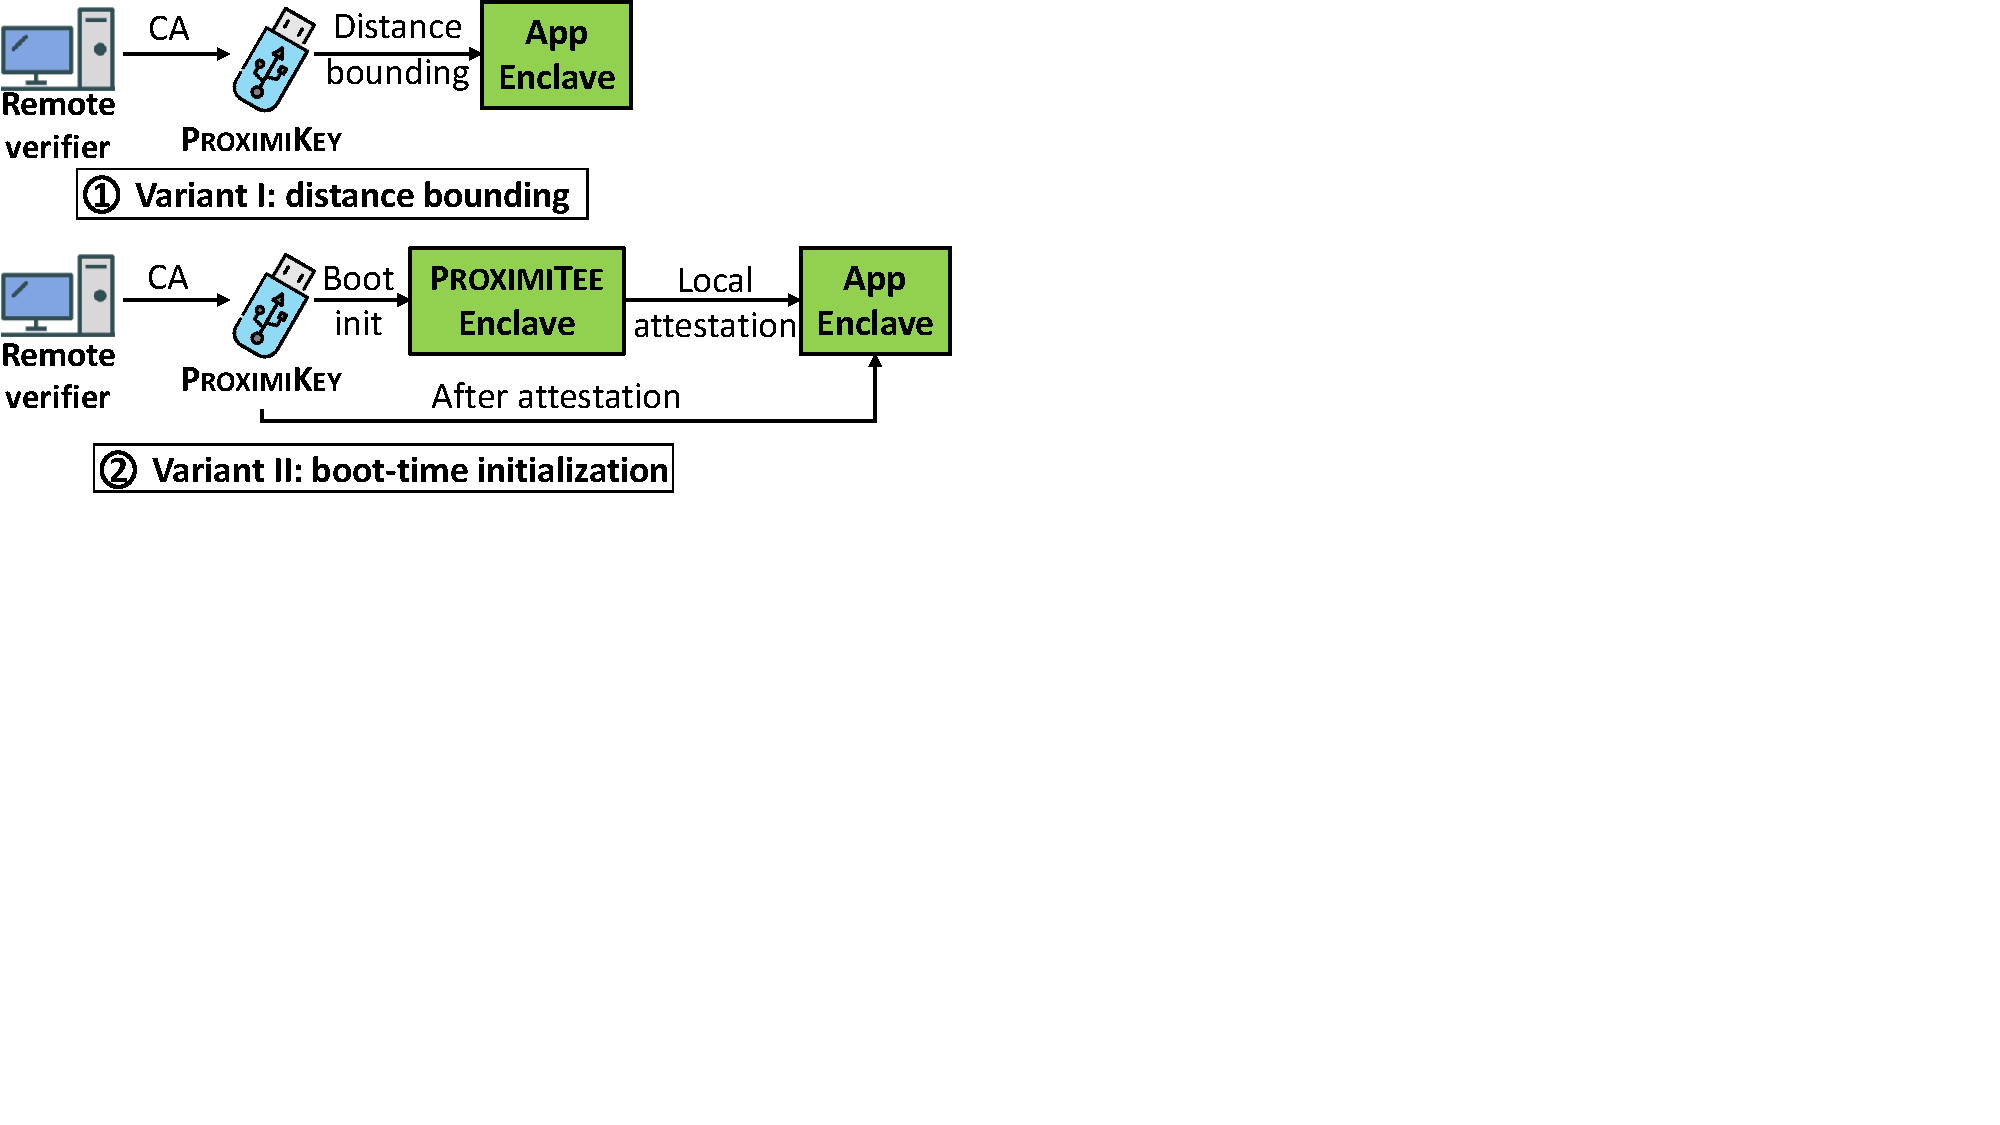
\includegraphics[trim={0 10.5cm 17cm 0},clip,width=0.88\linewidth]{TrustedPathComm.pdf}
  \else
  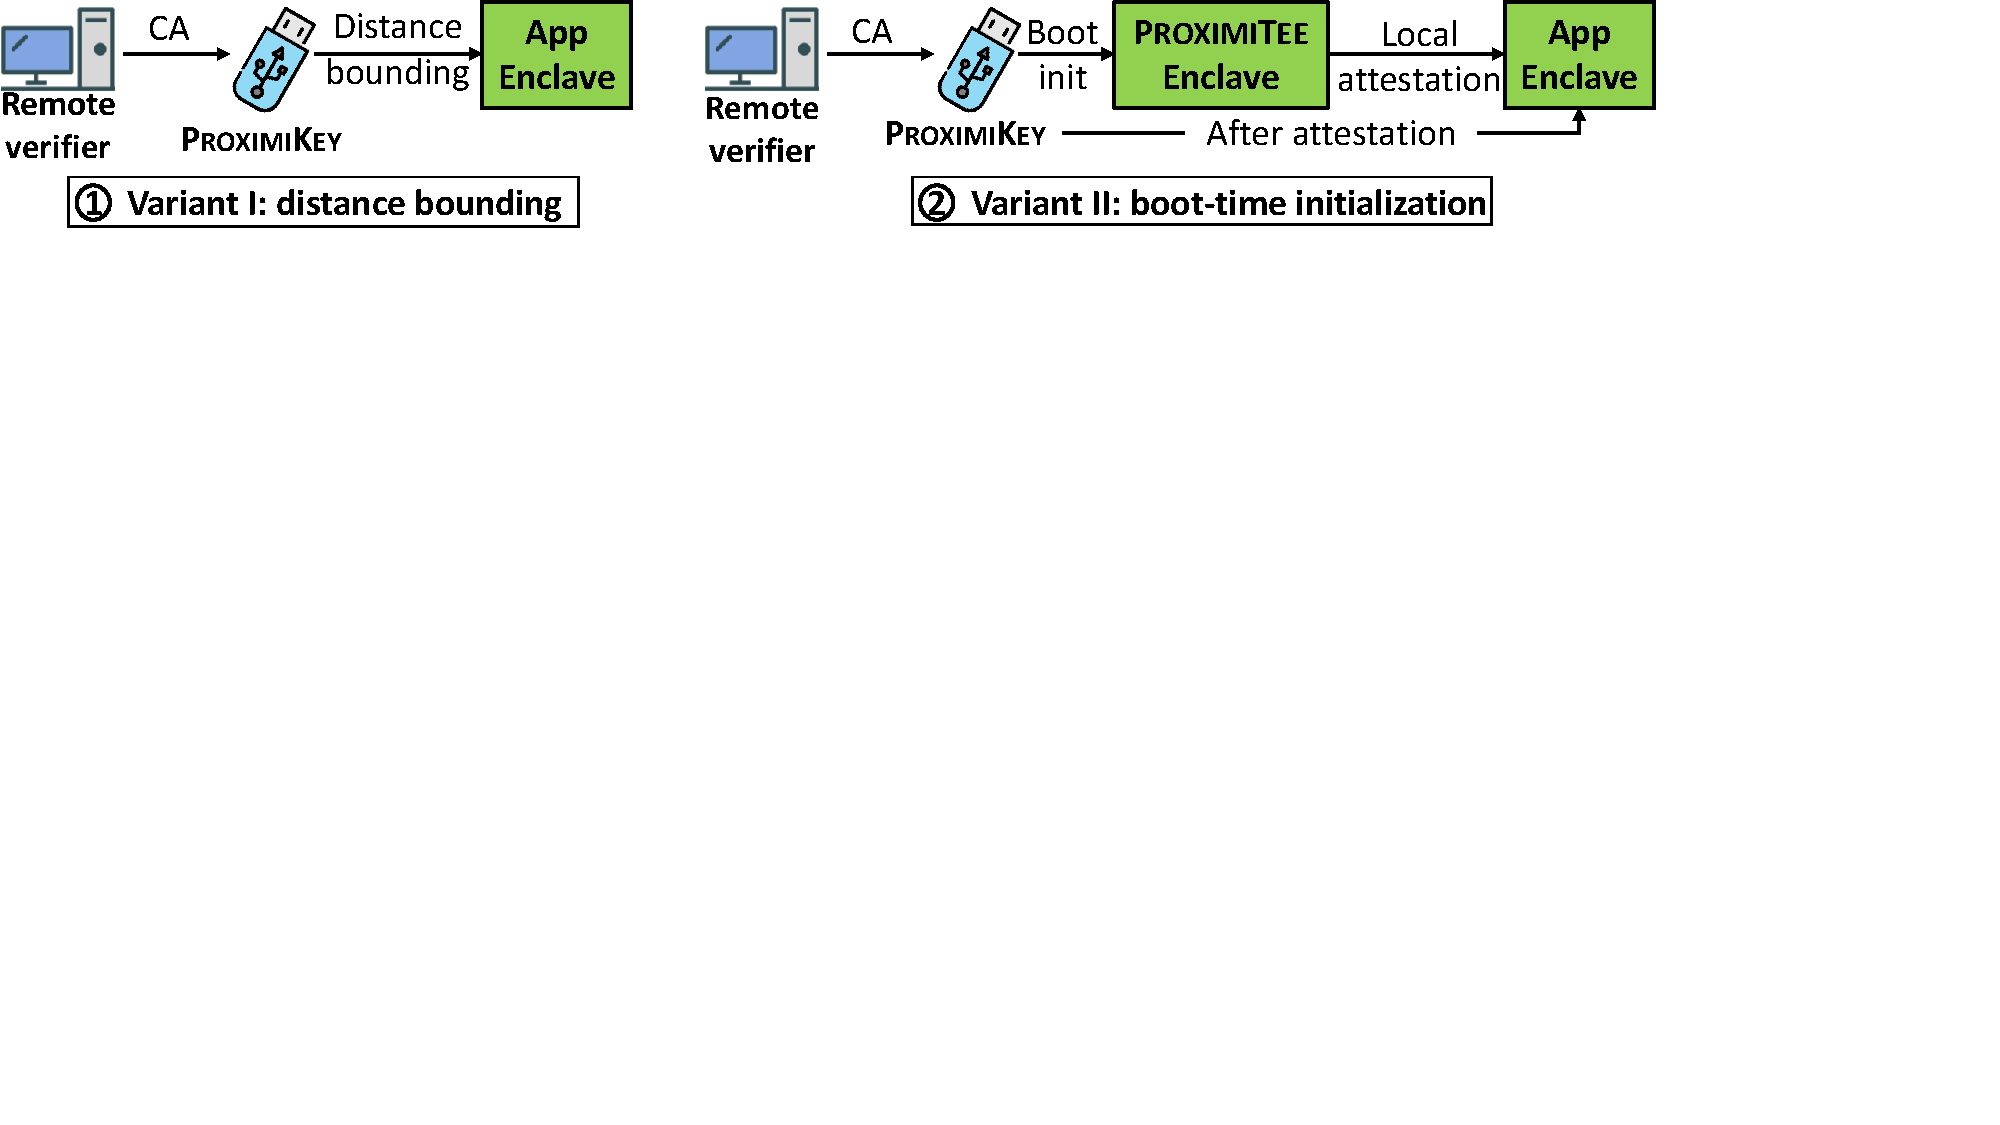
\includegraphics[trim={0 15cm 5cm 0},clip,width=0.95\linewidth]{TrustedPathComm_H.pdf}
  \fi 
 \caption{\textbf{Security analysis overview.} Attestation is successful, if the remote verifier establishes a secure communication channel to the correct enclave.}
 \ifusenix
 \vspace{-15pt}
 \else
 \fi
 \label{fig:trustedPathCommunication}
\end{figure}

The second subtask is to establish a secure connection from \device to the correct enclave. For this, we use proximity verification. \device verifies the proximity of the attested enclave through steps \five to \eight of the protocol. These steps essentially check two things. First, through step \seven, whether the messages are received from the correct enclave. This verification is performed by checking the correctness of the decrypted message, and it relies on the assumption that the attacker cannot break the underlying encryption and hence only the enclave that has access to the key that was bound to the attestation could have produced a valid reply. Second, through step \eight, whether the \device and the enclave are in each other's proximity. This check relies on the assumption that a reply from a remote enclave will take more time to reach the \device than a reply from the local enclave.

We evaluate the second aspect experimentally. In particular, we simulate a powerful relay-attack adversary that is connected to the target platform with short and fast network connection (one meter long Ethernet cable). Since the attacker's platform might be faster than the target platform, we simulate an adversary that can perform instantly all computation needed to participate in the proximity verification protocol. (The adversary cannot break cryptographic primitives such as encryption, hash, and signature.) We define adversary's success as the event where the proximity verification succeeds with an enclave that resides on the above-defined adversary's platform and denote the probability of such event $P_{adv}$. We define legitimate success as the event that proximity verification succeeds with a local enclave and denote its probability $P_{legit}$.

In Section~\ref{sec:evaluation} our experiments and analysis show that example parameter values $n=50$, $k=0.4$ and \connect$=470 \mu s$ enable reliable, secure and fast proximity verification. Proximity verification takes 25 ms, and therefore it adds only a minor delay to the initial attestation. The adversary's success probability is negligible: $P_{adv}=2.71\times 10^{-67}$. With the same parameters, proximity verification with the legitimate local enclave succeeds with a very high probability: $P_{legit}=0.999999965$. 

Since perfectly emulated SGX environment can pass any proximity test, this variant does not prevent emulation attacks enabled by leaked SGX attestation keys from other CPUs.

\ifusenix
\vspace{-14pt}
\else
\fi
\myparagraph{Mechanism II: Boot-time initialization.} Our second mechanism also prevents emulation attacks. This variant relies on the integrity of the BIOS / UEFI to run once per platform the correct \name kernel which initializes the \nameclave (there exist methods to verify the integrity of the BIOS/UEFI in hardware~\cite{titanchip}). 
% if for a particular scenario the administrator believes this prerequisite is not met.} 
The \name kernel is a single-purpose kernel that only supports a minimal set of features that is essential to run SGX which makes its attack surface small. 

In this variant, the task of establishing a secure communication channel to the correct enclave is broken into three subtasks (see the bottom in Figure~\ref{fig:trustedPathCommunication}). The first subtask is the same as above.

The second subtask is to establish a secure communication channel from \device to the \nameclave. For this, we use a secure boot-time initialization (i.e., trust on first use). \device shares a key with an enclave that is started by the trusted \name kernel, hence at a time in which the attacker could not emulate any enclave. \device knows when secure initialization takes place because the user (platform owner) indicates this by pressing a button which is an operation that the adversary cannot perform. The \nameclave seals the key during initialization. Different SGX CPUs cannot unseal each other's data, and therefore even if the adversary has extracted sealing keys from other SGX processors, she cannot unseal the key and masquerade as the legitimate \nameclave. %We leverage a crucial difference between an emulated enclave and a real enclave: the inability to unseal each other's data.

The third subtask is to establish a secure communication channel from the \nameclave to the \app. The security of this step relies on SGX's built-in local attestation functionality (see Appendix~\ref{sec:background} for details). An adversary in possession of leaked sealing attestation keys from other SGX processors, cannot produce a local attestation report that the \name enclave would accept, and therefore the adversary cannot trick the remote verifier to establish a secure communication channel to a wrong enclave.

\subsection{Periodic Proximity Verification Security}

To analyze the security of the periodic proximity verification that is used for platform revocation, we must first define what it means for the attacker to break the periodic proximity verification. The purpose of the periodic proximity verification is to prevent cases where the user detaches the \device from the attested target platform and attaches it to another SGX platform before the previously established connection is terminated. Since we consider an adversary who does not have physical access to the target platform (recall Section~\ref{sec:problemStatement:systemAttackerModel}), we focus on benign users and exclude scenarios where the \device would be connected to multiple SGX platforms with custom wiring or rapidly and repeatedly plugged in and out of two SGX platforms.

%\footnote{\blue{In principle, if the \device could be switched back and forth between two platforms, faster than the periodic proximity verification frequency and without losing power during the switch, periodic proximity verification would fail in detecting a disconnected device. If this attack is technically feasible, an attacker with physical access to the target platform could manage to provision data to a second machine while being undetected. Note that any information leaving \device will be encrypted with a key shared with an enclave in the target platform, so to make use of such data the attacker would also need to physically break the SGX protections in the target platform.}}

We define that adversary breaks the periodic proximity verification if the previously established connection is not terminated within a ``short delay'' after the \device was detached from the attested target platform. For most practical purposes we consider an example delay of 1 ms sufficiently short. We denote the adversary's success probability in breaking the periodic proximity verification as $P'_{adv}$.
%
False positive for periodic attestation is the event where the connection to the legitimate enclave is terminated and the attested platform is revoked despite the \device being connected to the platform. We denote the probability that this happens during a ``long period'' of usage as $P'_{fp}$. We consider an example period of 10 years sufficiently long for most practical usages.

In Section~\ref{sec:evaluation} evaluate this experimentally, again by simulating a similar relay-attack adversary. We show that there exists a set of parameters that provide secure, reliable and inexpensive channel termination and platform revocation. %$f=2000/s$, $w=20$, $k=0.3$ and  \detach$=649\mu s$
The attacker's success probability can be made negligible: $P'_{avd}=2.27\times10^{-64}$, while keeping the false positive probability low: $P'_{fp}=5\times10^{-5}$. Such periodic proximity verification consumes only $0.0011\%$ of the available channel capacity (\usb 2.0 has a channel capacity of $480$ MBits/s) between \device and the enclave, so we consider its cost minor.

%The attacker's success probability is measured based on the challenge-response latency distributions depicted in Figure~\ref{graph:reroutingDetectionHist}. The two timing distribution distinguishes a legitimate enclave running on the platform in proximity and the attacker's enclave running on the attacker's platform. For example, if the \name protocol is executed 10 per second continuously for $10$ years (24 hours a day and 365 days a year), the total number of trials would be $315.36 \times 10^7$. if the continuous \name protocol is executed with the sliding window of length $20$ (for the probability values refer to figure~\ref{graph:roundSuccess}), the probability of attacker's success probability will be $1.701 \times 10^{-10}$. the attacker's success probability is calculated as the standard error of mean from our experimental observation (more details in section~\ref{sec:evaluation:parameters}). If the user sets the number of rounds to even higher values, such as $50$ (where the attacker's success probability is $1.6\times 10^{-50}$, refer to Figure~\ref{graph:attackerSuccess}), the attacker's success probability over $10$ years will be $3.78\times10^{-41}$ which is negligible.


\subsection{TCB and Attack Surface}

Figure~\ref{fig:TOFU} illustrates a comparison of trusted components and attack surface between a TOFU solution where a trusted authority (CA) certifies enclave keys (cf.~Section~\ref{sec:problemStatement:limitations}) and our hardened attestation variants. In such TOFU solution, the TCB consists of the target platform hardware, the OS that needs to be trusted only at the time of first use, and a standard certification authority (CA). In our Variant I (distance-bounding), the TCB contains the target platform hardware, the embedded device (\device), and a CA that can be fully offline. The OS is untrusted. In our Variant II (boot-time initialization), the TCB contains the target platform hardware, the embedded device, an offline CA and a small kernel that needs to be trusted at the time of first use. This small kernel requires no network functionality, and thus this component can be considered offline.

\ifusenix
\begin{figure}[t]
 \centering
  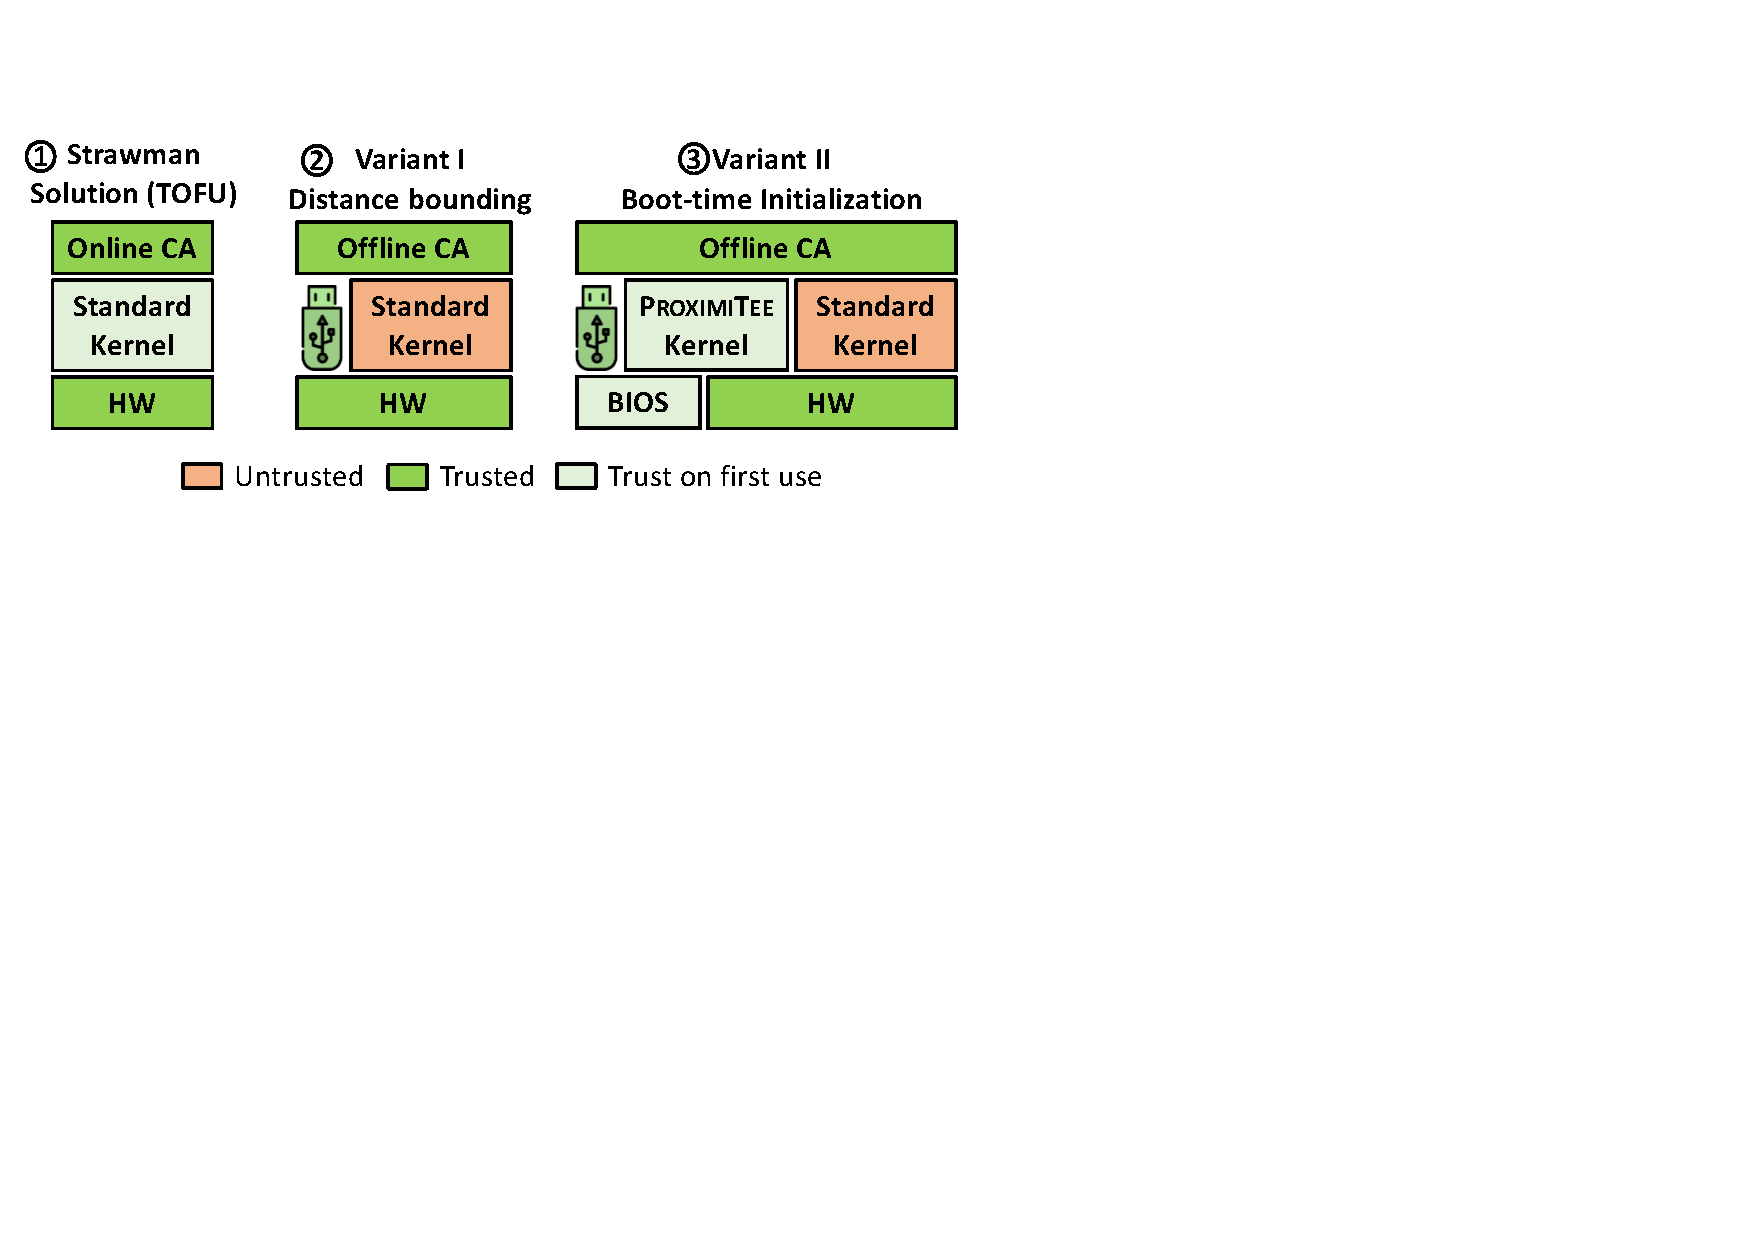
\includegraphics[trim={0 12.5cm 12.5cm 2cm},clip,width=0.9\linewidth]{TOFU1.pdf}
 \caption{\textbf{TCB comparison.} We illustrate the components that need to be trusted in our straw-man solution and two hardened attestation variants.}
 \vspace{-15px}
 \label{fig:TOFU}
\end{figure}

\else

\begin{figure}[t]
 \centering
  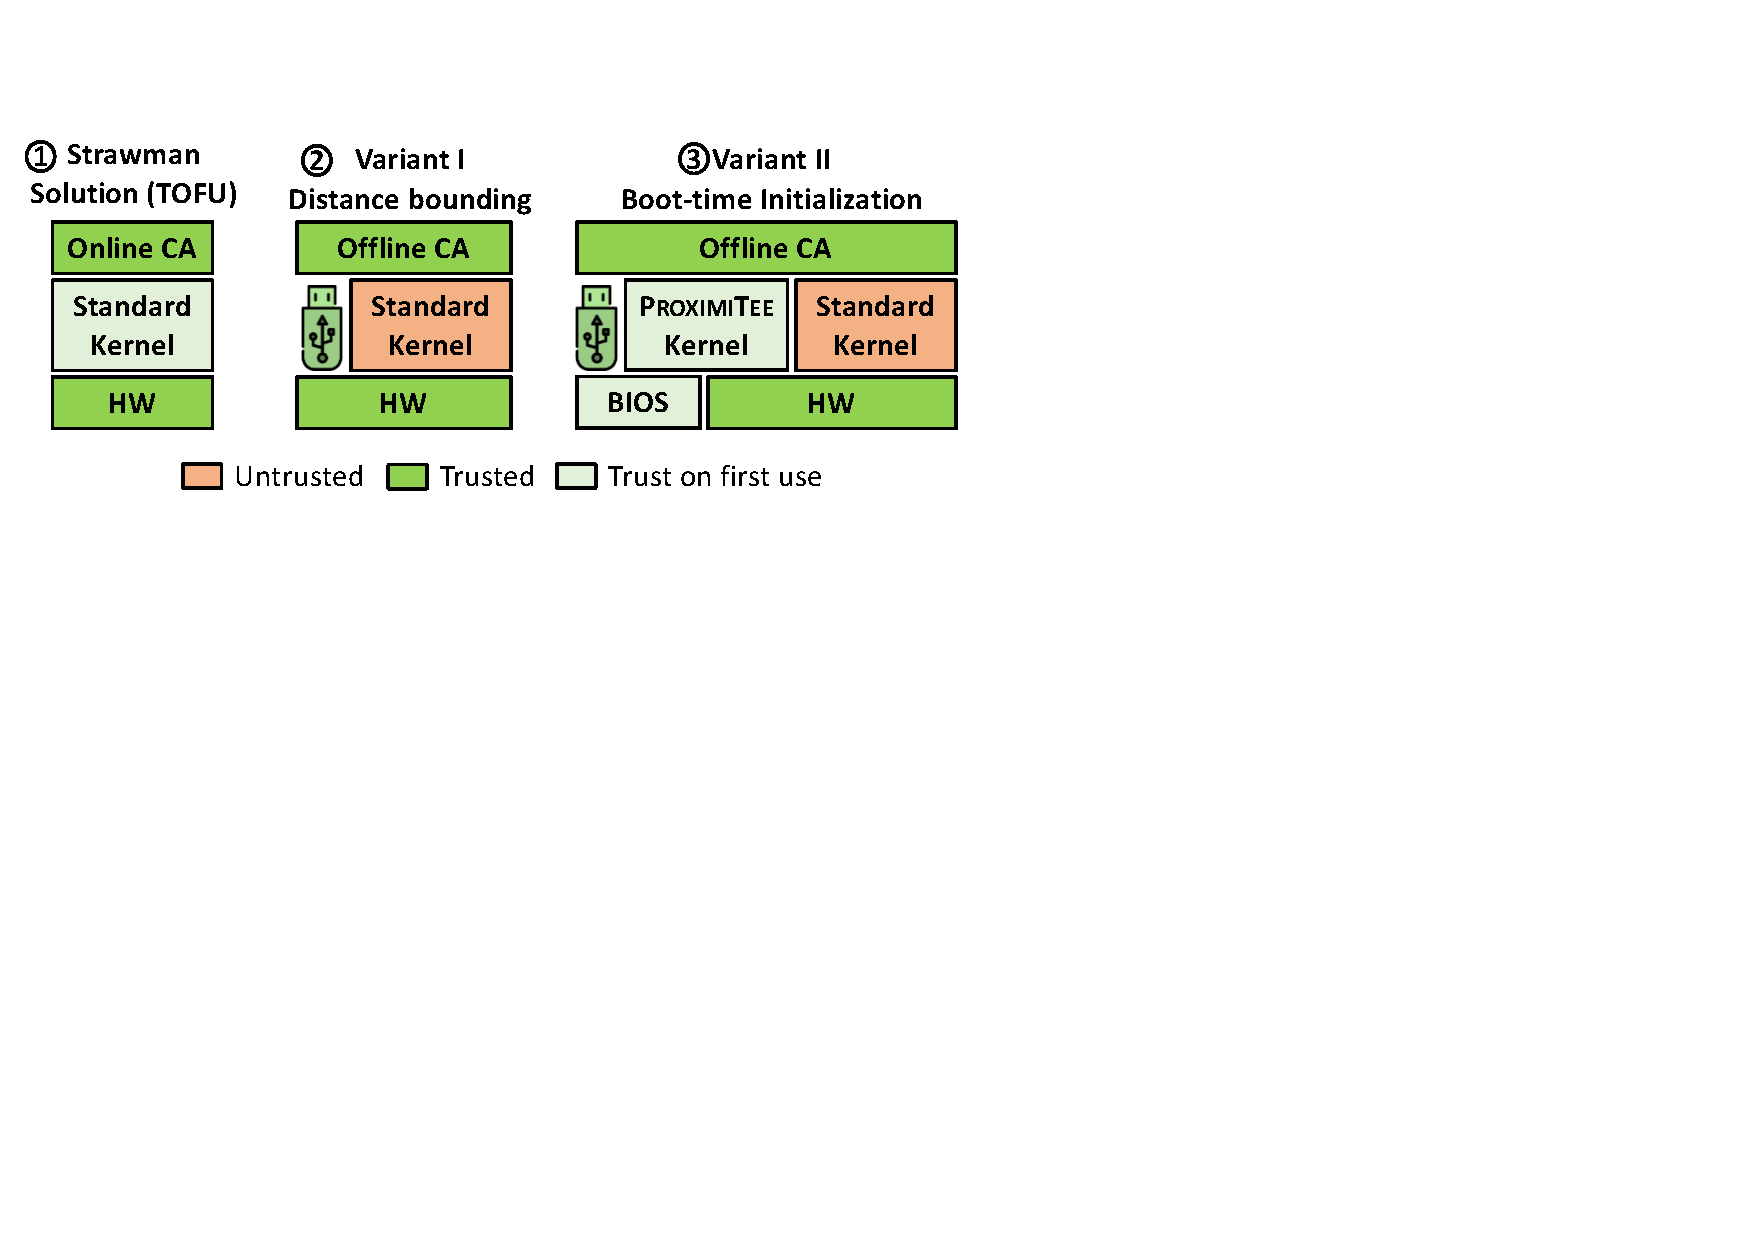
\includegraphics[trim={0 12.5cm 12.5cm 2cm},clip,width=0.6\linewidth]{TOFU1.pdf}
 \caption{\textbf{TCB comparison.} We illustrate the components that need to be trusted in our straw-man solution and two hardened attestation variants.}
 %\vspace{-25px}
 \label{fig:TOFU}
\end{figure}

\fi

In Section~\ref{sec:evaluation} we show that the complexity of our prototype implementation is small (3.6 KLoC) and thus both of our variants can provide significantly reduced TCB and attack surface over typical TOFU solutions.
